\documentclass{beamer}

\usetheme{AnnArbor}
\usecolortheme{dolphin}

\usepackage[utf8]{inputenc}
\usepackage[T1]{fontenc}
\usepackage{listings}
\usepackage{xcolor}
\usepackage{amsmath}
\usepackage{amssymb}
\usepackage{tikz}
\usepackage{pgfplots}

\pgfplotsset{compat=1.18}

\definecolor{codegreen}{rgb}{0,0.6,0}
\definecolor{codegray}{rgb}{0.5,0.5,0.5}
\definecolor{codepurple}{rgb}{0.58,0,0.82}
\definecolor{backcolour}{rgb}{0.95,0.95,0.92}

\lstdefinestyle{mystyle}{
    backgroundcolor=\color{backcolour},
    commentstyle=\color{codegreen},
    keywordstyle=\color{blue},
    numberstyle=\tiny\color{codegray},
    stringstyle=\color{codepurple},
    basicstyle=\ttfamily\small,
    breaklines=true,
    captionpos=b,
    keepspaces=true,
    numbers=left,
    numbersep=5pt,
    showspaces=false,
    showstringspaces=false,
    showtabs=false,
    tabsize=2
}

\lstset{style=mystyle}

\title{Introducción a la Geometría Espacial y Animación 3D}
\author{HCI}
\date{2026}

\begin{document}

\begin{frame}
\titlepage
\end{frame}

\begin{frame}{Objetivos}

\begin{itemize}
    \item Comprender el espacio tridimensional.
    \item Introducir la geometría espacial aplicada a gráficos 3D.
    \item Relacionar conceptos matemáticos en el contexto de raylib.
    \item Comprender el uso de la cámara en escenas 3D.
    \item Implementar geometría espacial y transformaciones utilizando raylib.
\end{itemize}

\end{frame}


\section{Sistema de Coordenadas 3D}

\begin{frame}{Sistema de Coordenadas 3D}

En geometría espacial los objetos existen en:

$$
(x,y,z)
$$

\vspace{0.3cm}

\begin{itemize}
    \item $x$ representa izquierda/derecha.
    \item $y$ representa arriba/abajo.
    \item $z$ representa profundidad.
\end{itemize}

\vspace{0.5cm}

Vector espacial:

$$
    \vec{v}=(x,y,z) \in \mathbb{R}^3
$$

\end{frame}

\begin{frame}{Representación del Espacio Tridimensional}

\begin{center}
\begin{tikzpicture}[scale=1.3]

\draw[->, thick, red] (0,0) -- (3,0) node[right] {$X$};
\draw[->, thick, green!70!black] (0,0) -- (0,3) node[above] {$Y$};
\draw[->, thick, blue] (0,0) -- (-2,-1.5) node[left] {$Z$};

\filldraw[black] (0,0) circle (2pt);

\node at (0.6,-0.4) {Origen $(0,0,0)$};

\end{tikzpicture}
\end{center}

\end{frame}

\begin{frame}[fragile]{Esqueleto Básico de un Programa 3D en raylib}

\begin{lstlisting}[language=C++,basicstyle=\ttfamily\tiny]
#include "raylib.h"

int main()
{
    InitWindow(1000, 700, "Escena 3D");

    Camera3D camera = { 0 };
    SetTargetFPS(60);

    while (!WindowShouldClose())
    {
        BeginDrawing();
        ClearBackground(RAYWHITE);

        BeginMode3D(camera);
            // Dibujar objetos 3D
        EndMode3D();

        EndDrawing();
    }

    CloseWindow();
    return 0;
}
\end{lstlisting}

\end{frame}

\begin{frame}{Interpretación del Ciclo de Animación 3D}

El programa funciona como un ciclo continuo de simulación y renderizado.

\vspace{0.5cm}

\textbf{1. Inicialización}

\vspace{0.2cm}

Se crean los elementos principales de la aplicación:

\begin{itemize}
    \item ventana,
    \item cámara,
    \item escena,
    \item variables de animación.
\end{itemize}

\vspace{0.5cm}

\textbf{2. Bucle principal}

\vspace{0.2cm}

El ciclo:

$$
while(!WindowShouldClose())
$$

mantiene activa la aplicación y permite actualizar continuamente la escena.

\end{frame}

\begin{frame}{Actualización y Renderizado}

\textbf{3. Actualización}

\vspace{0.2cm}

En esta etapa se modifican:

\begin{itemize}
    \item posiciones,
    \item velocidades,
    \item rotaciones,
    \item escalamiento,
    \item animaciones.
\end{itemize}

\vspace{0.5cm}

\textbf{4. Renderizado}

\vspace{0.2cm}

La GPU vuelve a dibujar toda la escena tridimensional.

\vspace{0.5cm}

Este proceso ocurre repetidamente para producir la ilusión de movimiento continuo.

\vspace{0.5cm}

Normalmente la animación se ejecuta a:

$$
60 \ \text{FPS}
$$

(60 cuadros por segundo).

\end{frame}



\begin{frame}[fragile]{3D en raylib}

\begin{lstlisting}[language=C++]
#include "raylib.h"

int main()
{
    InitWindow(1000, 700, "Sistema 3D");

    Camera3D camera = { 0 };

    camera.position = { 8.0f, 8.0f, 8.0f };
    camera.target = { 0.0f, 0.0f, 0.0f };
    camera.up = { 0.0f, 1.0f, 0.0f };

    SetTargetFPS(60);
}
\end{lstlisting}

\end{frame}

\begin{frame}{Interpretación Matemática de la Cámara}

La cámara posee una posición espacial:

$$
\vec{p}=(x,y,z)
$$

También posee una dirección visual:

$$
\vec{d}=\vec{target}-\vec{position}
$$

\vspace{0.4cm}

Esto permite construir la perspectiva del observador.

\end{frame}

\begin{frame}{Elementos Matemáticos de los Cuerpos 3D}

Los cuerpos geométricos tridimensionales poseen propiedades matemáticas que permiten describir:

\begin{itemize}
    \item dimensiones,
    \item volumen,
    \item superficie,
    \item posición espacial.
\end{itemize}

\vspace{0.2cm}

\textbf{Cubo}

$$
V=l^3
$$

\begin{itemize}
    \item $V$ representa el volumen.
    \item $l$ representa la longitud de cada lado.
\end{itemize}

\vspace{0.2cm}

\textbf{Esfera}

$$
V=\frac{4}{3}\pi r^3
$$

\begin{itemize}
    \item $V$ representa el volumen.
    \item $r$ representa el radio.
\end{itemize}

\end{frame}

\begin{frame}{Elementos Matemáticos del Cilindro}

\textbf{Cilindro}

\vspace{0.2cm}

El volumen de un cilindro se calcula mediante:

$$
V=\pi r^2 h
$$

donde:

\begin{itemize}
    \item $V$ representa el volumen.
    \item $r$ representa el radio de la base.
    \item $h$ representa la altura.
\end{itemize}

\vspace{0.1cm}

En gráficos 3D, estos parámetros permiten construir objetos geométricos con dimensiones controladas matemáticamente.

\vspace{0.1cm}

En raylib, el cilindro puede modelarse especificando:

\begin{itemize}
    \item posición,
    \item radio,
    \item altura,
    \item número de segmentos.
\end{itemize}

\end{frame}

\section{Transformaciones Geométricas}

\begin{frame}{Transformaciones Geométricas}

Las transformaciones permiten modificar objetos en el espacio.

\vspace{0.3cm}

Principales transformaciones:

\begin{itemize}
    \item Traslación.
    \item Rotación.
    \item Escalamiento.
\end{itemize}

\end{frame}

\begin{frame}{Traslación}

Mover un objeto en el espacio.

$$
\vec{p}'=\vec{p}+\vec{t}
$$

\vspace{0.5cm}

Donde:

\begin{itemize}
    \item $\vec{p}$ es la posición original.
    \item $\vec{t}$ es el vector de traslación.
\end{itemize}

\end{frame}

\begin{frame}[fragile]{Traslación en raylib}

\begin{lstlisting}[language=C++]
float x = -5.0f;

x += 0.03f;

DrawCube(
    { x, 1.0f, 0.0f },
    2.0f,
    2.0f,
    2.0f,
    BLUE
);
\end{lstlisting}

\end{frame}

\begin{frame}{Rotación}

La rotación modifica la orientación de un objeto.

\vspace{0.4cm}

Rotación sobre el eje Y:

$$
R_y(\theta)=
\begin{bmatrix}
\cos\theta & 0 & \sin\theta \\
0 & 1 & 0 \\
-\sin\theta & 0 & \cos\theta
\end{bmatrix}
$$

\end{frame}

\begin{frame}[fragile]{Rotación en raylib}

\begin{lstlisting}[language=C++]
rlPushMatrix();

rlTranslatef(0.0f, 1.0f, 0.0f);

rlRotatef(
    angulo,
    0.0f,
    1.0f,
    0.0f
);

DrawCube(
    {0.0f, 0.0f, 0.0f},
    2.0f,
    2.0f,
    2.0f,
    ORANGE
);

rlPopMatrix();
\end{lstlisting}

\end{frame}


\begin{frame}{Funciones de Rotación en raylib}

Para rotar objetos en raylib se utilizan funciones de la biblioteca \texttt{rlgl}.

\vspace{0.5cm}

\textbf{1. rlPushMatrix()}

\vspace{0.2cm}

Guarda temporalmente el sistema de transformación actual.

\vspace{0.3cm}

Esto permite aplicar transformaciones a un objeto sin modificar el resto de la escena.

\vspace{0.5cm}

\textbf{2. rlTranslatef(x,y,z)}

\vspace{0.2cm}

Desplaza el sistema de referencia hacia una nueva posición:

$$
(x,y,z)
$$

\vspace{0.2cm}

Este desplazamiento define el punto donde se realizará la rotación.

\end{frame}



\begin{frame}{Funciones de Rotación en raylib}

\textbf{3. rlRotatef(angulo,x,y,z)}

\vspace{0.2cm}

Aplica una rotación sobre un eje espacial.

\vspace{0.3cm}

Parámetros:

\begin{itemize}
    \item \texttt{angulo}: cantidad de rotación en grados.
    \item \texttt{(x,y,z)}: eje de rotación.
\end{itemize}

\vspace{0.4cm}

Ejemplo:

$$
(0,1,0)
$$

indica rotación sobre el eje \(Y\).

\vspace{0.5cm}

\textbf{4. rlPopMatrix()}

\vspace{0.2cm}

Restaura el sistema de transformación original de la escena.

\end{frame}


\begin{frame}{Idea Visual de \texttt{rlPushMatrix()} y \texttt{rlTranslatef()}}

\begin{center}
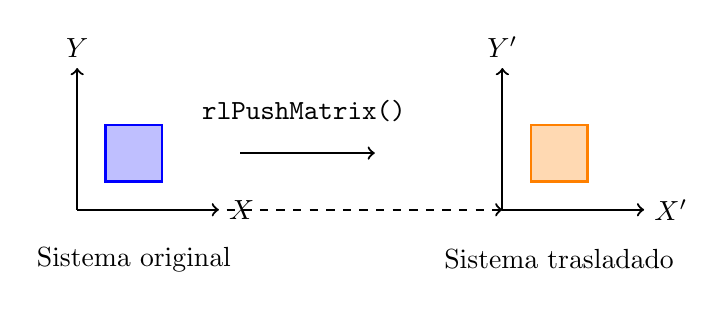
\begin{tikzpicture}[scale=0.9]

% Sistema original
\draw[thick, ->] (-5,0) -- (-3,0) node[right] {$X$};
\draw[thick, ->] (-5,0) -- (-5,2) node[above] {$Y$};

\draw[fill=blue!25, draw=blue, thick]
(-4.6,0.4) rectangle (-3.8,1.2);

\node at (-4.2,-0.7) {Sistema original};

% Flecha
\draw[->, thick] (-2.7,0.8) -- (-0.8,0.8);

\node at (-1.8,1.4)
{\texttt{rlPushMatrix()}};

% Sistema trasladado
\draw[thick, ->] (1,0) -- (3,0) node[right] {$X'$};
\draw[thick, ->] (1,0) -- (1,2) node[above] {$Y'$};

\draw[dashed, thick, ->] (-5,0) -- (1,0);

\draw[fill=orange!30, draw=orange, thick]
(1.4,0.4) rectangle (2.2,1.2);

\node at (1.8,-0.7) {Sistema trasladado};

\end{tikzpicture}
\end{center}

\vspace{0.4cm}

\begin{itemize}
    \item \texttt{rlPushMatrix()} guarda el sistema de referencia original.
    
    \vspace{0.3cm}
    
    \item \texttt{rlTranslatef(x,y,z)} desplaza el sistema de coordenadas hacia una nueva posición.
    
    \vspace{0.3cm}
    
    \item El objeto ahora se dibuja respecto al nuevo sistema trasladado.
\end{itemize}

\end{frame}

\begin{frame}{Idea Visual de \texttt{rlRotatef()} y \texttt{rlPopMatrix()}}

\begin{center}
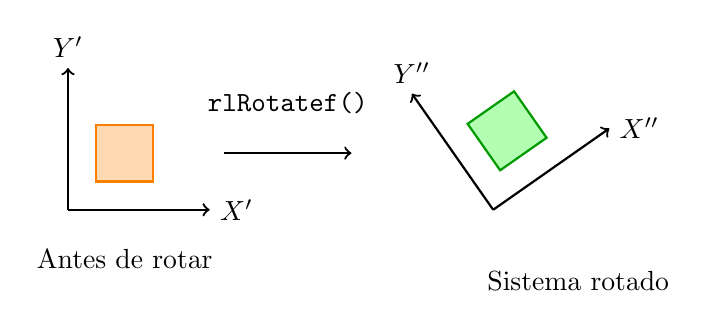
\begin{tikzpicture}[scale=0.9]

% Sistema trasladado
\draw[thick, ->] (-4,0) -- (-2,0) node[right] {$X'$};
\draw[thick, ->] (-4,0) -- (-4,2) node[above] {$Y'$};

\draw[fill=orange!30, draw=orange, thick]
(-3.6,0.4) rectangle (-2.8,1.2);

\node at (-3.2,-0.7) {Antes de rotar};

% Flecha
\draw[->, thick] (-1.8,0.8) -- (0.0,0.8);

\node at (-0.9,1.5)
{\texttt{rlRotatef()}};

% Sistema rotado
\begin{scope}[shift={(2,0)}, rotate=35]

\draw[thick, ->] (0,0) -- (2,0) node[right] {$X''$};
\draw[thick, ->] (0,0) -- (0,2) node[above] {$Y''$};

\draw[fill=green!30, draw=green!60!black, thick]
(0.4,0.4) rectangle (1.2,1.2);

\end{scope}

\node at (3.2,-1.0) {Sistema rotado};

\end{tikzpicture}
\end{center}

\vspace{0.4cm}

\begin{itemize}
    \item \texttt{rlRotatef()} rota el sistema de referencia del objeto.

    \vspace{0.3cm}

    \item La figura gira respecto al eje especificado.

    \vspace{0.3cm}

    \item \texttt{rlPopMatrix()} restaura el sistema original de la escena.
\end{itemize}

\end{frame}



\begin{frame}{Escalamiento Geométrico}

El escalamiento modifica el tamaño de un objeto tridimensional.

\vspace{0.5cm}

Geométricamente, cada coordenada del objeto se multiplica por un factor de escala.

\vspace{0.5cm}

$$
\vec{p}' = s\vec{p}
$$

\vspace{0.4cm}

donde:

\begin{itemize}
    \item $\vec{p}$ representa la posición original del punto.
    \item $\vec{p}'$ representa la nueva posición escalada.
    \item $s$ representa el factor de escala.
\end{itemize}

\vspace{0.5cm}

Interpretación:

\begin{itemize}
    \item si $s > 1$, el objeto crece.
    \item si $0 < s < 1$, el objeto disminuye.
    \item si $s = 1$, el tamaño permanece igual.
\end{itemize}

\end{frame}

\begin{frame}{Interpretación Espacial del Escalamiento}

Supongamos un cubo de tamaño:

$$
2 \times 2 \times 2
$$

\vspace{0.4cm}

Si aplicamos:

$$
s = 2
$$

entonces el nuevo tamaño será:

$$
4 \times 4 \times 4
$$

\vspace{0.5cm}

En raylib, el escalamiento se logra modificando dinámicamente:

\begin{itemize}
    \item ancho,
    \item altura,
    \item profundidad.
\end{itemize}

\vspace{0.5cm}

Esto permite crear animaciones donde los objetos parecen:

\begin{itemize}
    \item expandirse,
    \item comprimirse,
    \item respirar,
    \item pulsar.
\end{itemize}

\end{frame}


\section{Uso de Cámara}

\begin{frame}{La Cámara en Espacios 3D}

La cámara representa:

\begin{itemize}
    \item el observador,
    \item el punto de vista,
    \item la perspectiva.
\end{itemize}

\vspace{0.4cm}

Elementos principales:

\begin{itemize}
    \item position.
    \item target.
    \item up.
    \item fovy.
\end{itemize}

\end{frame}

\begin{frame}{Campo Visual de la Cámara}

El parámetro FOV representa:

$$
FOV = \text{Field Of View}
$$

\vspace{0.4cm}

\begin{itemize}
    \item FOV pequeño: efecto zoom.
    \item FOV grande: efecto panorámico.
\end{itemize}

\end{frame}

\begin{frame}[fragile]{Cámara Libre en raylib}

\begin{lstlisting}[language=C++]
UpdateCamera(
    &camera,
    CAMERA_FREE
);
\end{lstlisting}

\vspace{0.4cm}

La cámara puede:

\begin{itemize}
    \item moverse,
    \item rotar,
    \item explorar el espacio.
\end{itemize}

\end{frame}

\section{Animación Temporal}

\begin{frame}{Animación Temporal}

La animación consiste en modificar propiedades en función del tiempo.

\vspace{0.4cm}

Ejemplos:

\begin{itemize}
    \item movimiento senoidal,
    \item rebotes,
    \item órbitas,
    \item trayectorias.
\end{itemize}

\end{frame}


\begin{frame}{Movimiento Senoidal}

El movimiento senoidal modela oscilaciones periódicas.

\vspace{0.4cm}

Ejemplos físicos:

\begin{itemize}
    \item péndulos,
    \item ondas,
    \item vibraciones,
    \item movimiento armónico simple.
\end{itemize}

\vspace{0.5cm}

La posición vertical del objeto cambia según:

$$
y(t)=A\sin(\omega t)
$$

\vspace{0.4cm}

donde:

\begin{itemize}
    \item $y(t)$ representa la posición vertical.
    \item $A$ representa la amplitud máxima.
    \item $\omega$ representa la frecuencia angular.
    \item $t$ representa el tiempo.
\end{itemize}

\end{frame}

\begin{frame}{Interpretación Geométrica del Movimiento Senoidal}

La función seno produce un movimiento suave de subida y bajada.

\vspace{0.5cm}

Características:

\begin{itemize}
    \item cuando:
    
    $$
    \sin(\omega t)=1
    $$
    
    el objeto alcanza la altura máxima.
    
    \vspace{0.3cm}
    
    \item cuando:
    
    $$
    \sin(\omega t)=-1
    $$
    
    el objeto alcanza la altura mínima.
    
    \vspace{0.3cm}
    
    \item el movimiento se repite continuamente.
\end{itemize}

\vspace{0.5cm}

En raylib, este valor puede utilizarse para modificar dinámicamente la coordenada \(Y\) de un objeto.

\end{frame}


\begin{frame}{Movimiento Orbital}

El movimiento orbital describe trayectorias circulares alrededor de un centro.

\vspace{0.5cm}

Se modela utilizando funciones trigonométricas:

$$
x(t)=r\cos(t)
$$

$$
z(t)=r\sin(t)
$$

\vspace{0.5cm}

donde:

\begin{itemize}
    \item $r$ representa el radio de la órbita.
    \item $t$ representa el tiempo.
    \item $x(t)$ y $z(t)$ representan la posición del objeto.
\end{itemize}

\end{frame}

\begin{frame}{Interpretación Geométrica del Movimiento Orbital}

El objeto se desplaza alrededor de un punto central.

\vspace{0.5cm}

Geométricamente:

\begin{itemize}
    \item el coseno controla el desplazamiento horizontal.
    \item el seno controla el desplazamiento en profundidad.
\end{itemize}

\vspace{0.5cm}

La combinación simultánea de ambas funciones genera una circunferencia.

\vspace{0.5cm}

En gráficos 3D este movimiento se utiliza para:

\begin{itemize}
    \item planetas,
    \item satélites,
    \item cámaras orbitales,
    \item sistemas de animación.
\end{itemize}

\end{frame}

\begin{frame}[fragile]{Animación en raylib}

\begin{lstlisting}[language=C++]
float t = GetTime();

float x = cosf(t) * 4.0f;
float z = sinf(t) * 4.0f;

DrawSphere(
    {x, 1.0f, z},
    0.5f,
    RED
);
\end{lstlisting}

\end{frame}

\begin{frame}{Relación entre Matemáticas y Gráficos}

En gráficos 3D se utilizan:

\begin{itemize}
    \item álgebra lineal,
    \item geometría espacial,
    \item trigonometría,
    \item vectores,
    \item matrices.
\end{itemize}

\vspace{0.4cm}

Los motores gráficos convierten ecuaciones matemáticas en imágenes animadas.

\end{frame}

\begin{frame}{Conclusiones}

\begin{itemize}
    \item raylib facilita el aprendizaje de gráficos 3D.
    \item La geometría espacial es fundamental en simulación.
    \item La cámara define la percepción del espacio.
    \item Las transformaciones permiten animar objetos.
    \item Las matemáticas son la base de los gráficos por computador.
\end{itemize}

\end{frame}

\begin{frame}
\centering
\Huge
Gracias
\end{frame}

\end{document}
